\section{Transaction Lifecycle: From Execution to L1 Finality}
\label{sec:txlifecycle}

In this section, we describe the lifecycle of a transaction in zkSharding,
while highlighting specific solutions introduced to ensure both security
and efficiency.

In zkSharding, there are two fundamantal messages: external and internal
\handan{Does the naming make sense?}.  External messages originate from
external actors and are sent directly to the mempool of the contract’s
execution shard for processing. Internal messages, on the other hand, are
generated during contract execution and do not enter the mempool, as we
explained in Section \ref{sec:executionshards}. We differenciate internal
messages, for the sake of clarity in this section, as intra-shard
transactions (ISTs) and cross-shard transactions (CSTs) although ISTs and
CSTs share  the same structure and follow the similar execution path in
zkSharding.

Each internal message contains several fields that help process it
robustly,
but the key distinction between ISTs and CSTs lies in two specific fields:
the sender contract address $\sender$ and  the recipient contract address
$\to$.	To differentiate between shards, we use superscripts to denote
which shard the accounts belong to, e.g.,  $\sender^i$ and $\to^i$
indicate that  the sender or recipient account belongs to execution shard
$\shard_i$.
For a given transaction $\tx = (\sender^i, \to^j)$, if $i = j$, meaning
both the sender and recipient belong to the same shard, we classify it as
an \emph{intra-shard transaction (IST)}. If $i \neq j$, where the sender
and recipient belong to different shards, we classify it as a
\emph{cross-shard transaction (CST)}. In short:
\begin{itemize}
	\item ISTs are processed entirely in the execution shard where
	      they are initiated.
	\item CSTs involve interaction between different shards and
	      require cross-shard coordination.
\end{itemize}

Once either an internal or external message arrives to the execution
shard, it waits to be included in a block by a
block producer, who connects it to the blockchain, making it a canonical
part of the execution shard. Below, we describe this process in the
context of a block producer of $\shard_i$.

\subsection{Reaching Local Consensus}

\begin{figure}
	\centering
	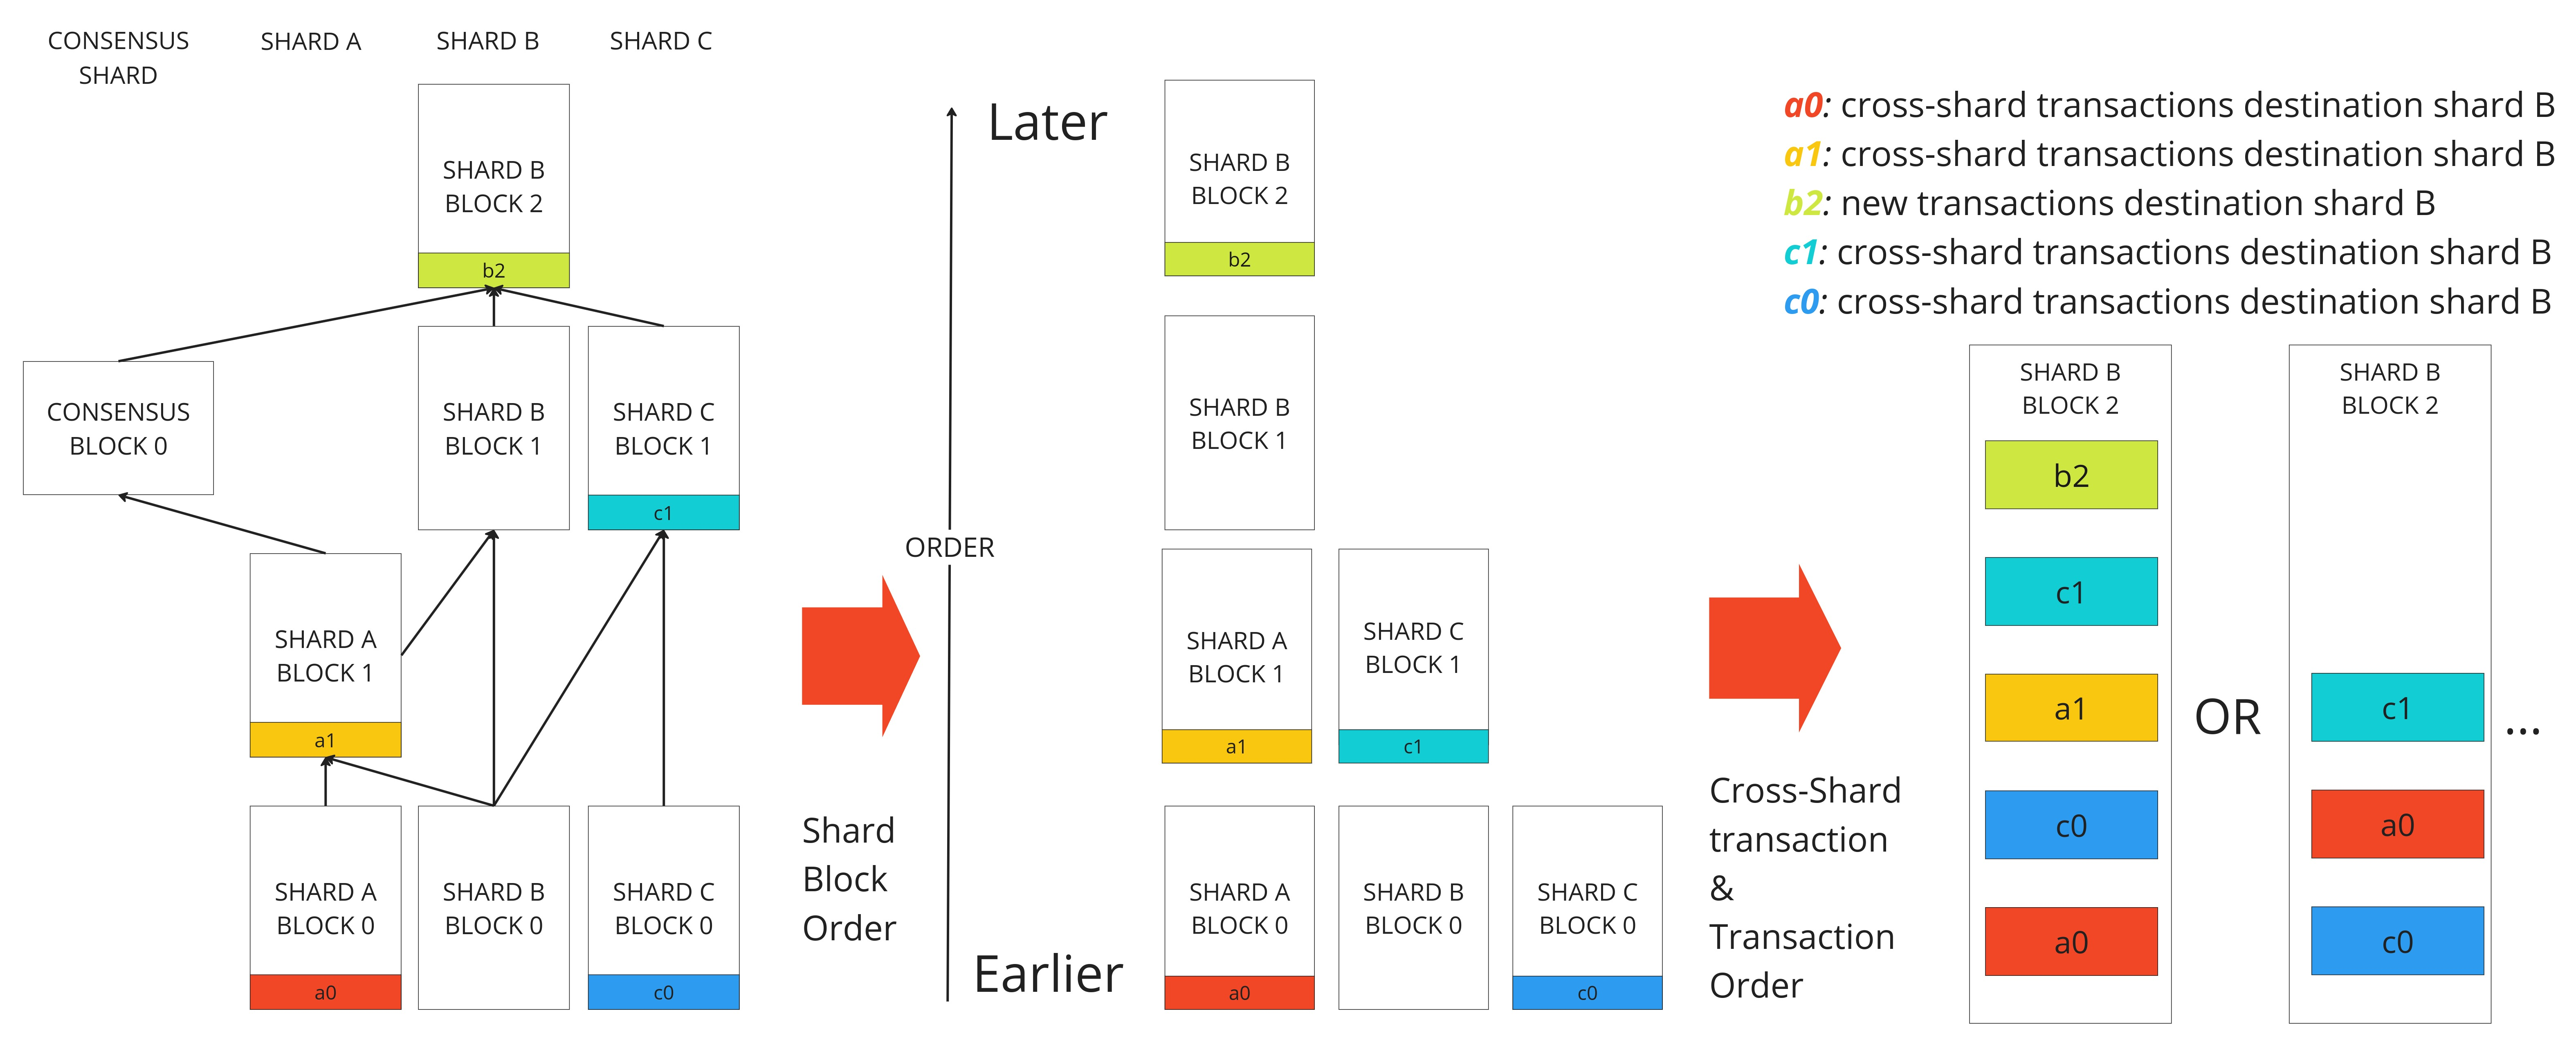
\includegraphics[width=1\linewidth]{figures/OrderExample}
	\caption{ShardDAG Order \handan{change notation and namings}}
	\label{fig:order}
\end{figure}
\begin{itemize}
	\item \textbf{Transaction ordering:}.
	      %, following transaction
	      %ordering rules based on factors such as \emph{fee}, \emph{priority},
	      %\emph{transaction type}, and  the \emph{ShardDAG ordering rules}.
	      The block producer begins by applying the ShardDAG ordering
	      rules (see Figure \ref{fig:order}). For this,
	      it first analyzes the local shardDAG subgraph for shard
	      $\shard_i$. This subgraph contains unprocessed transactions
	      $
		      \{(\sender^j, \to^i)\}$ where $j = i$ or $j \neq i$
	      and their dependencies
	      across different execution shards. The block producer then
	      determines the
	      order of these transactions with the help of the subgraph.
	      In case additional block space is available, it also selects
	      a set of
	      transactions from the mempool. In the end, it obtains the
	      list of transactions $\txlist$ to be processed.
	      The ShardDAG ordering rules enforce a \textit{parent-child
		      relationship} between transactions to be processed
	      in a valid order.
	      Specifically, CSTs with earlier dependencies must be
	      processed before
	      later transactions. This ordering prevents inconsistencies
	      in cross-shard
	      interactions.

	\item \textbf{Block Creation:} The proposer executes all
	      transactions in $ \txlist $ in the context of the latest
	      state using the
	      state transition function. If these executions
	      result in new cross-shard transactions
	      (CSTs), such as $ (\sender^i, \to^j) $ where $ i \neq j $,
	      the proposer
	      adds them to a special data structure called the
	      \emph{outbox} $ \outbox_i
	      $. $ \outbox_i $ tracks all CSTs originating from $ \shard_i
	      $ that are
	      waiting to be processed by their respective destination
	      shards\footnote{If
		      the block capacity is full and the mempool still
		      contains unprocessed messages  that should be
		      included based on the
		      ShardDAG order, they can be
		      added to the block's outbox for future inclusion in
		      later blocks
		      \cite{sharddag}}.

	      After executing the transactions, the block producer creates
	      a
	      block $ \block $. We note that if the execution of some CSTs
	      and ISTs fails, they enter a refund mechanism that allows
	      failed
	      transactions to be retried with additional fees or canceled
	      via the
	      mailbox.

	      \handan{It is not clear what solutions we use for the
		      failed CSTs. I am not sure whether what I wrote is
		      corret or not.}
	      When bulding $\block$, the block producer respects to the
	      Parent and Main-Parent condtions of ShardDAG rules.
	      Therefore, it
	      retrieves any new outgoing CSTs from other execution shards
	      and includes
	      the hashes of the originating blocks in $\block$, thereby
	      linking $\block$
	      to the corresponding blocks from other execution shards.
	      $\block$
	      includes the list of executed transactions $
		      \txlist $, the updated state $ \st $, state root
	      $\stroot$ of
	      $\st$, the outbox $ \outbox_i $, which contains CSTs that
	      are yet to be
	      processed by other shards and block header $\bhead$. This
	      newly created block is then proposed to
	      the network as part of the local consensus process.

	\item \textbf{Local Consensus:} After receiving the block $ \block
	      $, the validators initiate the Multi-Threshold BFT
	      \handan{Should we give the name of the consensus mechanism?
		      Maybe we
		      should not since it might change}
	      consensus mechanism \cite{MultiThresholdBFT} to validate and
	      finalize the
	      block \emph{locally} within execution shard $ \shard_i $.
	      Each validator
	      verifies the block’s correctness by \footnote{The list of
		      checks is not
		      exhaustive. We give the critical ones ensuring the
		      safety and security of
		      cross-shard communication.}
	      \begin{itemize}
		      \item verifying  the correctness of the transaction
		            order
		            in $\block$ to ensure that the order of
		            transactions adheres to the rules
		            of the shardDAG,
		      \item verifying if the block follows the parent
		            condition
		            and main-parent condition introduced by
		            ShardDAG rules and,
		      \item checking if $\fstf(\st', \txlist) \rightarrow
			            \st $
		            where $\st'$ is the last locally finalized
		            state.
	      \end{itemize}
	      Once a supermajority of validators  agrees on the
	      block's validity, the block is finalized locally.
	      This local consensus ensures that the block is securely
	      added to
	      $\shard_i $'s chain while maintaining consistency with the
	      shardDAG
	      ordering rules.
	      \short{
	      }{
		      The finalized block's header can then be propagated
		      to
		      other shards for further processing of CSTs as
		      described next.
	      }
	\item \textbf{Block Propogation:} After $\block$ is finalized
	      locally, validators are responsible for distributing $
		      \outbox_i $ and $ \bhead $ to the destination shards
	      $ \shard_j $, as well
	      as to other shards to ensure data availability of CSTs. They
	      are
	      incentivized to propagate the data to help reaching global
	      consensus at
	      the main shard level, as required by the child condition.
	      Remember that execution shards that receive the CST data
	      link
	      their next block to $ \bhead $. Even shards that do not
	      process the CSTs
	      must store the data off-chain, as they may be involved in
	      forming DAG
	      edges or verifying the ShardDAG rules, which is essential
	      for their own
	      block finality.

\end{itemize}

Validator sends $\bhead$ to the main shard after finalizing
it locally.

\subsection{Reaching the Global Consensus}
\label{sec:globalconsensus}

When the main shard validators receive a block header $\bhead$ from an
execution shard, they perform the following checks before including
$\bhead$ in a main shard block:

\begin{itemize}
	\item \textbf{Local Finality Check:} Confirm that $\bhead$ has
	      been signed by a supermajority of validators, indicating
	      that it has achieved local finality.
	\item \textbf{Validation of ShardDAG Rules:} Verify that the
	      \emph{Parent Condition}, \emph{Child Condition}, and
	      \emph{Main-Parent
		      Condition} are all satisfied. If
	      any of these conditions fail, the validators who signed
	      $\bhead$ are subject to slashing penalties.
\end{itemize}

If all checks pass, $\bhead$ is included in a main shard block and
finalized. If some of the checks are not passed, the validators signed for
$\bhead$ are slashed.

%However, at this stage,
%$\bhead$ is not yet fully recognized as a canonical part of $\shard_i$'s
%state because its state transition needs to be further verified.

%Once the synchronization committee (explained in the following section)
%submits a valid proof for a batch $\batch$ of transactions processed
%across all execution shards, the main shard validators update the status
%of $\bhead$ which has transactions in $\batch$ to \emph{finalized}. This
%step completes the process of achieving global consensus for $\bhead$ on
%$\shard_i$.
%
%Execution shards observing a pending $\bhead$ can infer that the CSTs
%included in the outbox of the block were correctly constructed according
%to ShardDAG rules and that the validators have agreed on
%the correct construction of the state. Thus, they can optimistically trust
%that $\stroot \in \bhead$ accurately represents the correct state $\st$
%without waiting for $\bhead$ to achieve global consensus on the main shard
%to process the CSTs.
%
%Our rotation algorithm, along with the high safety threshold of Multi-BFT,
%ensures that the safety of an execution shard is highly unlikely to be
%compromised. However, even in the rare case of a safety violation, we
%implement a rollback mechanism that ensures execution shards can revert to
%an uncorrupted state. Given the low probability of safety violations and
%the economic disincentives against attacking an execution shard, execution
%shards can rely on pending block headers to maintain continuity in their
%operations.

\subsection{Reaching the L1 Finality}

With the transactions now executed in an execution shard block and
included in the main shard, the next step involves the synchronization
committee $\syncSet$ to extract the transaction data, coordinate with
provers to generate proofs, and ultimately submit the verified data to L1
for final settlement and verification.
%In zkSharding, we have subset of validators that we call synchronization committee. This committee takes charge of extracting the transaction data, coordinating with provers to generate zk-proofs, and ultimately submitting the verified data to L1 for final settlement and verification. It is responsible for ensuring that the state changes and transactions from the execution shards are ready to be validated and posted to L1. 
Here is how  $\syncSet$\todois{not enough info on SC in the doc
	\handan{What else can I add? Maybe a motivation why we have such
		separate
		mechanism for it?}} executes
the process:

\begin{itemize}
	\item The \textbf{observer}\todois{From the text, it's not clear
		      what is the entity "observer" \handan{Not clear what
			      is not clear}} in $\syncSet$ monitors the
	      growth of the
	      main shard's state and execution shard states. Once the
	      state changes
	      reach a certain threshold, the observer initiates the
	      process of preparing
	      data for L1 submission.
	\item When the observer signals that a snapshot of data between
	      time $T$ (just after the last proven state) and $T + n$ is
	      ready, the
	      \textbf{aggregator} in $\syncSet$ compiles the data executed
	      between $T$
	      and $T+n$ in \emph{all} shards into a batch. Each batch of
	      $\shard_i$ consists of
	      transactions $\txlist_i$ executed between time $T $ and
	      $T+n$.
	      Addionally, the batch of the main shard consists of list of
	      transactions $\txlist_M$
	      between time $T$ and $T+n$ related to
	      % bridge operations such as
	      %withdrawal, depositing or 
	      validator operations such as staking, slashing
	      which are related the security of the internal sharding
	      mechanism. In the
	      end, aggregator composes	$k+1$ bathches where $k$ is the
	      number of
	      execution shard into one batch $\batch$.
	      The aggregator sends $\batch$, the last verified state on L1
	      $\st'$, and other necessary data to the verifier	in
	      $\syncSet$. It also forwards $\batch$ to the
	      proposer in $\syncSet$.
	      By grouping all transactions into a batch, we achieve better
	      cost-efficiency during the proving process.
	\item The \textbf{verifier} generates a special transaction called
	      \emph{proof order} to outsource the proof generation process
	      to the prover
	      network.	The proof order specifies the batch and state
	      updates that need
	      to be proven, along with a payment for generating the proof.
	      Prover
	      network runs the proving algorithm which receives as a
	      private input
	      $\batch$, current state $\st'$ and as a public input
	      %$\combatch$ which is
	      %the commitment of $\batch$ and 
	      the new state root $\stroot$ and previous
	      verified state root $\stroot'$. In simple terms, provers
	      generate a succinct proof $\pi$ that verifies the
	      correctness of the new
	      state with the public inputs (See Section \ref{sec:l1} to
	      understand the
	      proving statement).

	      %	       (part of) our proving
	      %	      system runs for the following relation $\mathcal{R}_\fstf$:
	      %
	      %	      \begin{align*}
	      %		      \mathcal{R}_\fstf = & \{((\batch, \st'); (\combatch,
	      %		      \stroot, \stroot')):  \mtroot(\st) \rightarrow \stroot, \mtroot(\st')
	      %		      \rightarrow \stroot'                                                      \\ \nonumber
	      %		                          & \fstf(\st',\batch) \rightarrow \st, \commit(\batch)
	      %		      \rightarrow \combatch \}
	      %	      \end{align*}
	      %
	      %	      where $\commit$ is a commitment algorithm and $\mtroot$ is an
	      %	      algorithm that outputs the Merkle Tree root of a given state.
	      %	      In the end, our proving algorithm outputs a proof $\pi$ if
	      %	      $((\batch, \st'); (\combatch, \stroot, \stroot')) \in \mathcal{R}_\fstf
	      %	      $. 
	      After receiving $\pi$, the verifier gives
	      $\pi$ to the proposer if $\pi $ is verified.
	      The provers joining the proving process get their fee.
	\item The \textbf{Proposer} runs the compression algorithm
	      for $\batch$ which is an optimized algorithm
	      for zkSharding’s specific data types (e.g., block headers,
	      state roots,
	      and transaction summaries). This reduces the size of the
	      data submitted to
	      L1. Once the batch is compressed, the proposer submits it to
	      L1 through an
	      EIP-4844 blob transaction. This transaction includes the
	      compressed batch
	      data. The blob transaction ensures that the data is
	      permanently
	      stored and its KZG commitment $\kzg$ is accessible for
	      future
	      verification.
	      Addionally, the proposer submits $\pi$ and public inputs to
	      the
	      L1 state validity contract and the main shard.
\end{itemize}

Once the L1 State Validity Contract verifies $\pi$ as described in Section
\ref{sec:l1}, it updates the verified state root to $\stroot$ and
finalizes it as part of L1 through Casper FFG. It means that once a state
is finalized  through Casper FFG, it is irreversible and considered as a
canonical part of  Ethereum and also zkSharding.

\handan{Add motivation why we have distinct roles within the sync
	commitee, why do we we have many members, how the roles are
	distributed.}